% !TEX root = ../my-thesis.tex
%
\selectlanguage{english}  
\chapter{\textcolor{ctcolormain}{
Colonization pattern of abandoned croplands by \Qp in a Mediterranean mountain region}}\label{sec:coloniza}


\mbox{}
\vfill
{\color{ctcolormain}\textbf{Antonio J. Pérez-Luque}}; Francisco J. Bonet-García \& Regino Zamora 
2021. \emph{Forests}, 12 (11): 1584. \href{https://dx.doi.org/10.3390/f12111584}{doi:10.3390/f12111584}


\newpage

\paragraph{Abstract} \mbox{} \\
Land abandonment is a major global change driver in the Mediterranean region where anthropic activity has played an important role shaping landscape configuration. Understanding the woodland expansion towards abandoned croplands is critical to develop effective management strategies. In this study we analyze the colonization pattern of abandoned croplands by \Qpy in Sierra Nevada mountain range (southern Spain). We aimed to assess differences among populations within the rear-edge of the \Qp distribution. For this purpose we characterized \emph{(i)} the colonization pattern of \Qp, \emph{(ii)} the structure of the seed source (surrounding forests), and \emph{(iii)} the abundance of the main seed disperser (Eurasian jay, \emph{Garrulus glandarius}). The study was conducted in five abandoned croplands located in two representative populations of \Qp located in contrasting slopes. Vegetation plots within three habitat-types (mature forest, edge-forest and abandoned cropland) were established to compute the abundance of oak juveniles. Abundance of European jay was determined using data of bird censuses (7-year). Our results indicate that a natural recolonization of abandoned croplands by \Qp is occurring in the rear edge of the distribution of this oak species. Oak juvenile abundance varied between study sites. Neither surrounding-forest structure nor the abundance of jays varied significantly between study sites. The differences in the recolonization patterns seem to be related to differences in the previous- and post abandonment management.
\newpage

\section{Introduction}\label{sec:coloniza:intro}

Land-use change is considered the main global change driver worldwide \autocites{Butchartetal2010GlobalBiodiversity,Winkleretal2021GlobalLand} affecting biodiversity \autocites{Sala2000GlobalBiodiversity}, modifying ecological processes \autocites{Lindenmayeretal2012LandUse}, and altering the provision of ecosystem services \autocites{Hasanetal2020ImpactLand}. Croplands abandonment and afforestation are the main processes of land-use change in the Northern hemisphere \autocites{Winkleretal2021GlobalLand,ReyBenayas2007AbandonmentAgricultural}. In Mediterranean region, where anthropic activity has played an important role shaping landscape configuration, cropland abandonment has been widespread during the second half of the last century \autocites{Piasetal2014ColonizationAbandoned,ValbuenaCarabanaetal2010HistoricalRecent,MartinezFernandezetal2015RecentLand}. Land-use change models predict an increase in this trend in the future \autocites{Rounsevelletal2006CoherentSet,PerpinaCastilloetal2021ModellingAgricultural}. The abandonment of traditional activities has left many Mediterranean landscapes in an almost barren state, with poor vegetation cover \autocites{Sheffer2012ReviewDevelopment, ReyBenayas2007AbandonmentAgricultural}. Consequently, a natural vegetation regeneration process started with a spontaneously recovery of abandoned croplands \autocites{Debusscheetal1999MediterraneanLandscape,PenuelasBoada2003GlobalChangeinduced,AlvarezMartinezetal2014InfluenceLand,Nataleetal2007StudyTree,Piussi2000ExpansionEuropean}. 

Thus, the abandonment of traditional uses since the middle of the last century \autocites{MacDonaldetal2000AgriculturalAbandonment}, has caused a decrease in anthropogenic pressure on Mediterranean forest ecosystems \autocites{ValbuenaCarabanaetal2010HistoricalRecent}, being particularly important for mountain areas \autocites{Nataleetal2007StudyTree, AlvarezMartinezetal2014InfluenceLand,JimenezOlivenciaetal2015MedioSiglo,Piasetal2014ColonizationAbandoned}. The dramatic rural exodus occurred in mountain areas due to changes in socio-economic conditions \autocites{EuropeanEnvironmentAgency2010EuropeEcological}, resulting an abandonment of traditional activities and significant environmental changes \autocites{MacDonaldetal2000AgriculturalAbandonment, Nataleetal2007StudyTree, AlvarezMartinezetal2014InfluenceLand,Piussi2000ExpansionEuropean,Rutherfordetal2008AssessingLanduse,Zimmermannetal2010EffectsLanduse}. Moreover the abandonment of mountain agricultural areas is causing an increase in forest expansion via the spontaneous recovery of vegetation \autocites{Piussi2000ExpansionEuropean, AlvarezMartinezetal2014InfluenceLand}, that can causes a homogenization of the landscape \autocites{Mietkiewiczetal2017LongtermChange} with several ecological consequences \autocites{Zimmermannetal2010EffectsLanduse}. 

\begin{figure}[]
    \centering
    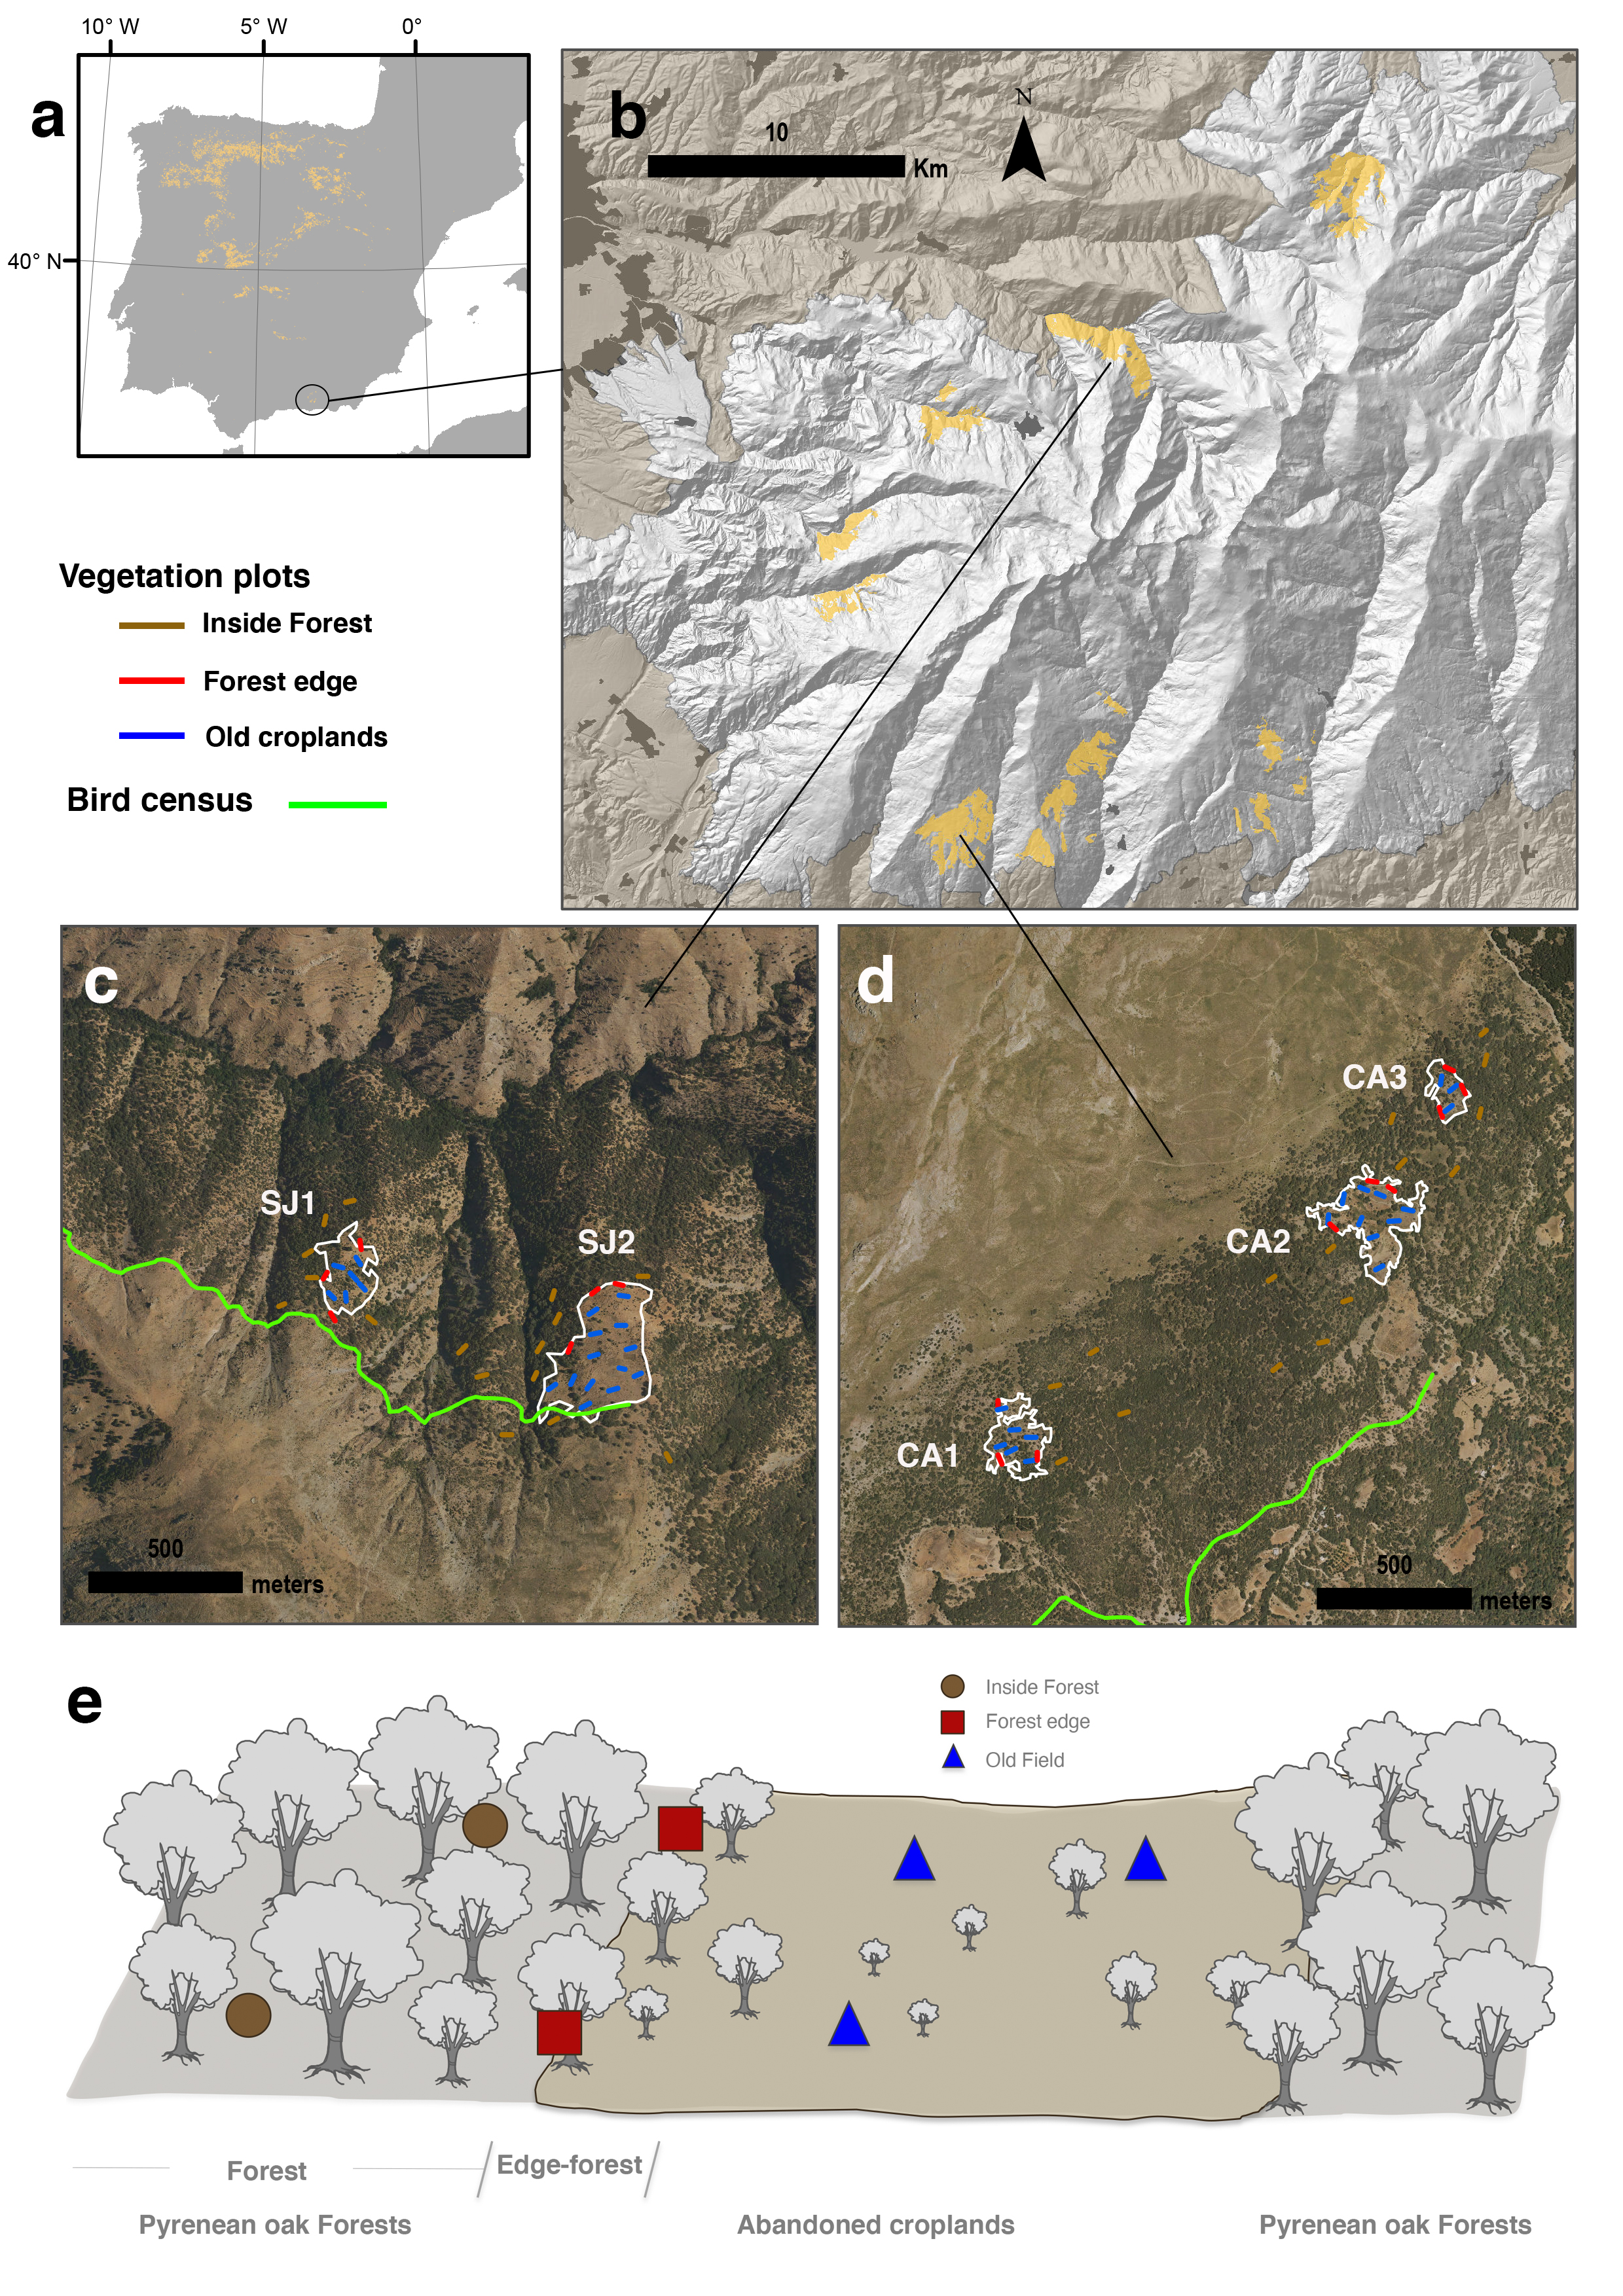
\includegraphics[width=\textwidth,height=16cm,
  keepaspectratio]{img/coloniza/coloniza-map.jpg}
    \caption{Distribution of \Qp forests in the Iberian Peninsula (a), and in Sierra Nevada mountain range (b). Location of the old croplands (\emph{white} lines) in the study sites: Robledal de San Juan (SJ) (c), and Robledal de Cáñar (CA)(d). Names of the old croplands as in \tabref{tab:coloniza:croplands}. Sampling design (e). Vegetation plots were randomly placed in the abandoned croplands (triangles), and inside the forest (circles) surrounding the old field. Several plots were also located at forest-old field edge (squares).}
    \label{fig:coloniza:transects}
\end{figure}


\Qpw woodlands, like other forest formations in the Mediterranean region, have been subjected to intense anthropogenic pressures over time \autocites{GarciaJimenez20099230Robledales, AlbaSanchezetal2021EarlyAnthropogenic}, which have led to the reduction of their distribution area, as well as to the modification of their floristic and structural patterns \autocites{Gavilanetal2000EffectsDisturbance,Calvoetal1999PostfireSuccession,Tarregaetal2006ForestStructure}. Historically, the woodlands of \Qp have been exploited mainly for firewood, charcoal, and tannins \autocites{RuizdelaTorre2006FloraMayor,SanchezPalomaresetal2008EstacionesEcologicas}. Some areas were also burned and thinned to create pastures with low densities of mature trees that provide acorns, firewood, and large areas for grazing \autocites{HerreraCalvo2016UsoPastoral,Alvarezetal2009CambiosEstructura,ValbuenaCarabanaGil2017CentenaryCoppicing}. All these anthropogenic processes have transformed the oak woodlands in a deep way that it is difficult to find stands that can be considered natural forests \autocites{RuizdelaTorre2006FloraMayor}. Nonetheless, the decrease in anthropogenic pressure has paradoxically caused that many of the \Qp oak stands present a state of advanced degradation, showing growth stagnation, lack of fruiting, and also symptoms of branch dieback  \autocites{Canellasetal2004GrowthResponse, Bravoetal2008SelviculturaMontes, ValbuenaCarabanaGil2014EfectosGestion, PiqueVericat2015EvolutionPerspectives, Piqueetal2018Spain}. 

Therefore, understanding the woodland expansion towards abandoned croplands would become critical to develop effective management strategies, particularly for populations representing the rear-edge of their distribution \autocite{HampePetit2005ConservingBiodiversity} which need a particular attention due to their high conservation value \autocite{Fadyetal2016EvolutionbasedApproach}.  
The study of ecological dynamics within the rear-edge populations is considered essential to establish proper management guidelines under current climate uncertainties \autocites{Fadyetal2016EvolutionbasedApproach,Jumpetal2010MonitoringManaging}. Rear-edge populations are often adapted to local environmental conditions at the limit of the species ecological amplitude, and often show a long-term persistence \autocite{HampePetit2005ConservingBiodiversity}. Local responses to environmental changes may differ from the species mean response \autocites{Benavidesetal2013DirectIndirect,Matiasetal2017ContrastingGrowth,Castroetal2004SeedlingEstablishment}, and such differences may either promote or hamper the survival of edge populations under global change \autocites{Fadyetal2016EvolutionbasedApproach,Jumpetal2010MonitoringManaging}. In this work we analyze the colonization pattern of abandoned croplands by \Qpy in Sierra Nevada mountain region. This mountain has undergone significant land use changes in the last 50 years \autocites{JimenezOlivenciaetal2015EvolucionUsos} with increases of forest densities \autocite[see chapter \ref{sec:carbon}; also][]{JimenezOlivenciaetal2015MedioSiglo}, and tree growth \autocite[see chapter \ref{sec:dendro};][]{PerezLuqueetal2020LanduseLegacies}. We are interested in exploring the colonization pattern of abandoned croplands by \Qp on both slopes of the Sierra Nevada. We aimed to assess differences among populations in the rear edge of its distribution. Our specific goals are \emph{(i)} to analyze the colonization pattern of abandoned cropland by \Qp and its relationship with time after abandonment; \emph{(ii)} to explore differences on the structure of the seed source (mature woodlands); and \emph{(iii)} to compare the abundance of the main seed disperser (Eurasian jay, \emph{Garrulus glandarius}).

\section{Material and Methods}\label{sec:coloniza:MatMet}
\subsection{Sampling description}\label{sec:coloniza:sampling}

\begin{table}
\caption{Main characteristics of the abandoned croplands studied.}
\centering
\resizebox{\linewidth}{!}{
\begin{tabular}[t]{cc>{\centering\arraybackslash}p{8em}ccccc}
\toprule
\multicolumn{1}{c}{ } & \multicolumn{2}{c}{Cropland} & \multicolumn{2}{c}{ } & \multicolumn{3}{c}{Number of plots} \\
\cmidrule(l{3pt}r{3pt}){2-3} \cmidrule(l{3pt}r{3pt}){6-8}
Site & Code & Abandonment Age (years) & Elevation (m) & Area (ha) & Cropland & Edge & Forest\\
\midrule
 & CA1 & > 60 & 1796-1866 & 3.29 & 6 & 3 & 4\\
\cmidrule{2-8}
 & CA2 & < 30 & 1789-1858 & 5.80 & 9 & 3 & 7\\
\cmidrule{2-8}
\multirow{-3}{*}{\centering\arraybackslash Robledal de Cáñar} & CA3 & 40 - 60 & 1851-1892 & 1.56 & 3 & 3 & 4\\
\cmidrule{1-8}
 & SJ1 & 40 - 60 & 1507-1674 & 3.47 & 6 & 3 & 6\\
\cmidrule{2-8}
\multirow{-2}{*}{\centering\arraybackslash Robledal de San Juan} & SJ2 & 30 - 40 & 1575-1746 & 10.36 & 13 & 3 & 10\\
\bottomrule
\end{tabular}}
\label{tab:coloniza:croplands}
\end{table}

We sampled 5 abandonment croplands located at two Pyrenean oak forests in contrasting slopes of Sierra Nevada (southern Spain): Robledal de San Juan (SJ), located at the northern aspect (37°7'29.63"N, 3°21'54.60"W; Güejar-Sierra, Granada, Spain); and Robledal de Cáñar (CA), located at the southern aspect (37°57'28.04"N, 3°25'57.1"W; Cáñar, Granada). We selected oak populations located at contrasting slopes since differences in environmental variables have been reported for those oak woodlands \autocite{PerezLuqueetal2021EcologicalDiversity}. Each cropland was delimited using land-use and land-cover map of Andalusia for 1956 \autocites[][]{CMA2007MapaUsos} combined with a detailed photographic interpretation of the black and white 1956 orthophotos (1-m spatial resolution) \autocites[see][for more details]{NavarroGonzalezetal2012CartografiaHistorica}. The estimation of the age abandonment for each cropland were performed combining intrepretation of orthophotographies with information from local neighbors. We compiled all available aerial ortophotographies of the study areas from Fototeca Digital of the Spanish National Geographic Institute (\href{http://fototeca.cnig.es/}{http://fototeca.cnig.es/}). These dates were verified using information about past land-use, compiled from local neighbours \autocites[by local workshops and interviews with retired elder: farmers, shepherds and loggers; see details in ][]{MorenoLlorcaetal2014CaracterizacionFuentes,MorenoLlorcaetal2016HistoricalAnalysis}. The estimated rank of ages could be considered accurate (see \tabref{tab:coloniza:croplands}).

For each abandonment cropland, vegetation plots (30 m x 10 m) were randomly distributed in the old field; at the forest edges; and inside the surrounding forests (\figref{fig:coloniza:transects}). The number of plots within the old fields and surrounding forests were proportional to the size of the abandonment cropland (\tabref{tab:coloniza:croplands}). A total of 83 vegetation plots were sampled in autumn 2012. In each vegetation plot all tree species were recorded, and tree height and diameter were measured. For each transect we computed the juvenile abundance as the number of individuals smaller than 150 cm on height. We did not distinguish the reproductive and vegetative origins of young oaks, since it is difficult due to the resprouting trait of this species. In addition to the juvenile abundance, we explored differences between several recruitment stages based on individual size \autocites[\emph{e.g}][]{Plieningeretal2010LargeScalePatterns}. We considered five size categories based in height (every 30 cm). All data were properly documented and published in an international repository \autocites[see][for a detailed description of the dataset]{PerezLuqueetal2015DatasetMIGRAME}. 
To explore the main bird disperser in our study sites, we used bird censuses carried out by the Sierra Nevada Global Change Observatory (\href{https://obsnev.es/}{https://obsnev.es/}). This dataset contains bird censuses at different ecosystems types of Sierra Nevada since 2008 \autocites[for more details see][]{BareaAzconetal2012PasseriformesOtras, PerezLuqueetal2016DatasetPasserine}. We only used data for the Eurasian jay (\emph{Garrulus glandarius}), since it is the main disperser of \Qpy \autocites{Gomez2003SpatialPatterns}. We assumed that jays can move acorns into abandoned croplands based on the habitat-preferences to cache acorns reported by \citet{PonsPausas2007AcornDispersal}, and also considering preliminary data on jays flights carried out in our study sites by \citet{Zamoraetal2013CambioGlobal}, who found a high proportion of flights of this bird at the same elevation, and around 40\% of open areas as arrival habitat. Since we were interested in the comparison of the Eurasian jay populations between the two study sites, we computed the annual bird abundances (in terms of birds/10 ha) for each site during a 7-year period (2008-2013). The sampling procedures was the line-transect method with a bandwith of 50 m (25 m on each side). Transects length were 2.80 km for Cáñar site (CA), and 3.22 km for San Juan site (SJ). Sight and sound records within the sample area were accepted as contacts. All transects were sampled in the early morning. Eurasian jay abundance was calculated in terms of birds/10 ha. All counts in one month were averaged, and the yearly result was obtained from the average of all the months studied. For more details about bird censuses see \citet{BareaAzconetal2012PasseriformesOtras} and \citet{ZamoraBareaAzcon2015LongTermChanges}.


\subsection{Data analysis}\label{sec:coloniza:analysis}
We used the vegetation plots carried out inside the forest (habitat type = forest) to analyze the structure of the seed source (surrounding forest). Several parameters related to forest structure and functioning were computed: tree density, juvenile abundance, tree species composition, tree size related statistics (\emph{i.e.} mean, median, maximum, 75 and 90 percentiles of tree-height), and basal area (BA). Differences between sites were assessed using the non-parametric Mann–Whitney U-test, since data did not meet normality nor/either homocedasticity assumptions. We also compared whether there was variation within plots belonging to the same sites. ANOVA analyses were performed to explore differences of bird disperser abundance (\emph{G. glandarius}) between sites and across years. 

The variation of the juvenile abundance between study sites, habitat type, and their interaction (site-habitat type), was analyzed using Generalized Linear Models with a Tweedie distribution with a log link \autocite{DunnSmyth2018TweedieGLMs}. Study sites and habitat type were the explanatory variables. Prior to the analysis, data exploration was applied following protocols described by \citet{Zuuretal2010ProtocolData} and \citet{IenoZuur2015BeginnerGuide}. As the dataset comprised count data, we initially used the Poisson and the Negative Binomial distribution. However, these models were overdispersed. A variance power parameter of 1.28 (1.20-1.40, 95\% confidence interval) were used in the Tweedie GLM model. This parameter was estimated using the \texttt{tweedie.profile} function of the \texttt{tweedie} R package \autocites{DunnSmyth2005SeriesEvaluation,Dunn2017Tweedie}. Model comparison (univariate models) was carried out using the Akaike's information criterion (AIC) \autocites{BurnhamAnderson2010ModelSelection}. The model accuracy was tested by Nagelkerke's pseudo-$R^2$, used as a measure of goodness of fit. The significance of the explanatory variables in the selected model was tested using the likelihood ratio tests (LRT). Wald z-tests and Tukey's HSD-corrected \emph{post hoc} comparisons were used to test for differences in juvenile abundance among sites and habitat-type. 

\begin{table}
\caption{Forest attributes of northern (SJ) and southern (CA) sites. U Mann-Withney statistics with significance at 0.05 level. Mean and SE are shown}
\centering
\resizebox{\linewidth}{!}{
\begin{tabular}[t]{ccccc}
\toprule
Variable & Southern site (CA) & Northern site (SJ) & U statistic & p value\\
\midrule
\% of Q. pyrenaica & 96.11 ± 1.28 & 100 ± 0 & 3.688 & 0.0001\\
Tree density (ind/ha) & 1671.11 ± 229.21 & 1587.5 ± 161.67 & 4.808 & 0.9369\\
Juvenile abundance (ind/ha) & 1004.44 ± 195.72 & 883.33 ± 127.18 & 4.852 & 0.7667\\
Adult abundance (ind/ha) & 584.44 ± 80.47 & 704.17 ± 63.31 & 4.448 & 0.1780\\
Maximum tree height (m) & 13.93 ± 0.65 & 13.75 ± 0.71 & 4.824 & 0.8736\\
Tree height mean (m) & 4.32 ± 0.6 & 5.09 ± 0.37 & 4.330 & 0.0855\\
Tree height median (m) & 3.19 ± 0.83 & 3.57 ± 0.66 & 4.564 & 0.3527\\
Tree height 75 percentile (m) & 5.73 ± 1.02 & 8.29 ± 0.6 & 4.343 & 0.0922\\
Tree height 90 percentile (m) & 10.07 ± 0.95 & 11.22 ± 0.54 & 4.605 & 0.4399\\
Basal Area (m2/ha) & 37.56 ± 4.23 & 33.58 ± 3.6 & 4.912 & 0.5400\\
\bottomrule
\end{tabular}}
\label{tab:coloniza:forest}
\end{table}

\begin{table}[]
\caption{Model selection for the oak juvenile abundance, sorted by minimum AICc value.}
\resizebox{\textwidth}{!}{%
\begin{tabular}{@{}llllll@{}}
\toprule
\textbf{model.name} & \textbf{df} & \textbf{logLik} & \textbf{AICc} & \Delta \textbf{AICc} & \textbf{Nagelkerke R\textsuperscript{2}} \\ \midrule
Habitat type + Site + Habitat type \(\times\) Site & 6 & -221.89 & 457.78 & 0 & 0.970 \\
Habitat type + Site & 4 & -231.83 & 473.65 & 15.87 & 0.955 \\
Habitat type & 3 & -236.21 & 480.42 & 22.64 & 0.946 \\
Site & 2 & -291.06 & 588.12 & 130.34 & 0.116 \\
null model & 1 & -293.09 & 590.19 & 132.41 & 0 \\ \bottomrule
\end{tabular}%
}%
\label{tab:coloniza:modelselection}
\end{table}

\section{Results}\label{sec:coloniza:results}

The forest structure of \Qpy woodlands did not show significant differences for the forest attributes between study sites  (\tabref{tab:coloniza:forest}). \Qpy woodlands of southern site (CA) showed higher tree density but smaller tree heights (mean, median and percentiles) than those on the northern site (SJ) (\tabref{tab:coloniza:forest}). In addition, higher abundance of juveniles was found for CA site, which also showed greater basal area than SJ site (\tabref{tab:coloniza:forest}).

Regarding the abundance of \emph{Garrulus glandarius}, no differences between study sites were found (\(F_{1,82}\) = 2.387; p = 0.126; CA = 1.69±0.21 and SJ = 1.33±0.22 birds/10ha), neither across years in the studied period (2008-2014) (\(F_{6,82}\) = 1.234; p = 0.297). The interaction term was also not significant (\(F_{6,82}\) = 1.26; p = 0.284).

\begin{figure}[H]
    \centering
    \includegraphics[width=\textwidth,height=8cm,
  keepaspectratio]{img/coloniza/coloniza-juvenile-interaction.pdf}
    \caption{Interaction plot for the oak juvenile abundance. Habitat-type differences within each site were indicated with different letters. Differences between sites for each habitat-type were indicated with asterisk. CA: \emph{Robledal de Cáñar} site (southern slopes); SJ: \emph{Robledal de San Juan} site (northern slopes).}
    \label{fig:coloniza:interaction}
\end{figure}

The juvenile oak abundance model including all terms (\emph{i.e.} full model) showed higher strength of empirical support than did models for each of the independent variables (\emph{i.e.} univariate models) (\tabref{tab:coloniza:modelselection}). Oak juvenile abundance differed among habitat types (\(F_{2,77}\) = 72.95; p < 0.0001), and between study sites (\(F_{1,77}\) = 8.16; p = 0.0054; \tabref{tab:coloniza:anova}). 

A decreasing gradient of oak-juvenile abundance was found across habitat-type, from higher values in forest type (15.90 ± 1.30 \juv) to lower values inside the old croplands (2.43 ± 0.55 \juv; \figref{fig:coloniza:interaction}). The abundance of oak juveniles in the old croplands of the southern site (CA) was significantly higher (4.06 ± 0.98 \juv) than in those of the northern site (SJ; 0.90 ± 0.26 \juv). 

The size distribution of juveniles was also different among the study sites (\figref{fig:coloniza:treeCategory}). An even size-distribution of the oak juveniles was observed in the old croplands of northern site. Conversely, higher contribution of small oak juveniles (< 30 cm) were found at old croplands of southern site (\figref{fig:coloniza:treeCategory}). 

A positive relation was found between the oak juvenile abundance and the estimate age of crop abandonment (\figref{fig:coloniza:ageCrop}) with higher oak juvenile abundances in the earlier abandoned croplands 

\section{Discussion}\label{sec:coloniza:disussion}

\begin{table}
\footnotesize
\caption{ANOVA table of the selected GLM model for the abundance of \Qpy juvenile across study sites and habitat types. F-value and p-values are displayed.}
\centering
\begin{tabular}{lllll} 
\toprule
\textbf{Variable}        & \textbf{SS} & \textbf{df} & \textbf{F} & \textbf{p-value}  \\ 
\midrule
Habitat type             & 233.89      & 2           & 72.95      &  0.0001           \\
Site                     & 13.09       & 1           & 8.16       & 0.0054            \\
Habitat type $\times$ Site & 27.19       & 2           & 8.48       & 0.0004            \\
Residuals                & 123.43      & 77          &            &                   \\
\bottomrule
\end{tabular}
\label{tab:coloniza:anova}
\end{table}


We observed a colonization process of \Qpy into abandoned croplands in this mountain region despite the strong recruitment constraints described for this species \autocites{Bravoetal2008SelviculturaMontes,Gomez2003ImpactVertebrate,Pereaetal2014InteraccionesPlantaanimal}. Forest expansion towards abandoned croplands has been recorded in several marginal habitats in other European mountainous regions \autocites{Amezteguietal2016LanduseLegacies,Nataleetal2007StudyTree,Piussi2000ExpansionEuropean,Amezteguietal2010LanduseChanges,LasantaMartinezetal2005MountainMediterranean,Kozak2003ForestCover,AlvarezMartinezetal2014InfluenceLand,VicenteSerranoetal2004AnalysisSpatial}, as consequence mainly of rural depopulation and decrease on herbivores pressure \autocite{MacDonaldetal2000AgriculturalAbandonment,EuropeanEnvironmentAgency2016EuropeanForest}. Our results show a relationship between juvenile-oak abundance and the estimated age of crop abandonment (\figref{fig:coloniza:ageCrop}). As the time after crop abandonment increases, species heterogeneity and functional diversity of the ecosystem increases \autocites{PuertaPineroetal2012HistoryMatters,HermyVerheyen2007LegaciesPresentday}, boosting the multifuntionality of the ecosystems \autocite{CruzAlonsoetal2019LongTerm}. 

\begin{figure}
    \centering
    \includegraphics[width=\textwidth,height=10cm,
  keepaspectratio]{img/coloniza/coloniza-TreeCategory.pdf}
    \caption{Juvenile abundance classified by tree-size (see material and methods) by habitat-type in the two study sites. Mean and standard error are shown.}
    \label{fig:coloniza:treeCategory}
\end{figure}

It has been also reported that both age of the surrounding forests and previous land use could influence the colonization pattern \autocite{MinottaDegioanni2011NaturallyRegenerated}. In this sense, it is expected that the colonization process will continue, since the forests surrounding our study areas are relatively young. Dendrochronological estimates of the forest age for our study woodlands, ranged approximately 90-100 and 200 years for northern and southern oak populations respectively \autocite{PerezLuqueetal2020LanduseLegacies, GeaIzquierdoCanellas2014LocalClimate}, which is younger than the estimated ages for these forests along their distribution range \autocites{GeaIzquierdoCanellas2014LocalClimate}. \citet{CruzAlonsoetal2019LongTerm}, in a study of the recovery of multifunctionality in Mediterranean forests, reported for this oak species, a minimum of 80 years after the abandonment for the recovery of the reference multifunctionality. 

The colonization pattern of abandoned croplands varies within the rear-edge of the \Qp. Our results showed different abundances of oak juveniles between sites, with higher abundances at the southern sites (CA) (\tabref{tab:coloniza:anova}; \figref{fig:coloniza:interaction}). It is known that the distance to the source and the structure of the seed source influenced the propagule input into new habitats \autocites{Nathan2006LongDistanceDispersal,HewittKellman2002TreeSeed,Kureketal2019DispersalDistance}. In our study sites, all the abandoned croplands are surrounded by native forests. Thus, the observed differences in oak juvenile abundance would not seem explained by the distance to the seed source (\tabref{tab:coloniza:croplands}). Regarding to the structure of the seed source, we found no differences between the study sites (\tabref{tab:coloniza:forest}). Forest attributes potentially related to the acorn production \autocite[\emph{e.g.} tree density, basal area,][]{GeaIzquierdoetal2006AcornProduction} are not different for surrounding forests between study sites (\tabref{tab:coloniza:forest}). Although in our work we have not carried out an estimation of acorn production that would allow us to compare between study sites, previous studies analyzing the variation in reproductive parameters and comparing the acorn production across oak woodlands of Sierra Nevada, found slight differences among oak populations, with higher acorn yield for southern oak woodlands than northern one \autocite{Leal2013AnalisisCrecimiento}.  However, the data series used by \citet{Leal2013AnalisisCrecimiento} was very short (only two years) and \Qpy have a marked mast-seeding behaviour \autocites{Bravoetal2008SelviculturaMontes,Gomezetal2001ProblemasRegeneracion}. Besides that, there not seem to be marked differences in the current seed source that could explain our observed differences in the abundance of juveniles in the abandoned crops. 

\begin{figure}
    \centering
    \includegraphics[width=\textwidth,height=6cm,
  keepaspectratio]{img/coloniza/coloniza-ageCrop.pdf}
    \caption{Relation of the juvenile oak abundance with the estimated age of crop abandonment.}
    \label{fig:coloniza:ageCrop}
\end{figure}

Another key aspect for the tree colonization of abandoned croplands is the dispersion vectors. \Qp acorn are mainly dispersed by woodmouse (\emph{Apodemus sylvaticus}) and Eurasian jay (\emph{Garrulus glandarius})\autocites{Gomez2003ImpactVertebrate,Pereaetal2014InteraccionesPlantaanimal}. We used a time series (a 7-year period) to analyze the abundance of jays at each study site. The aim of using this time series was to explore whether there were differences between study sites with respect to the abundance of this bird acorn-disperser. We are aware of the limitation of using these data, \emph{i.e.} we do not know if the abundance of jays at both sites has followed the same temporal trajectory, but we have used the longest time series we have for both sites, to at least find out if there are differences between the sites in recent years. Our results showed similar abundances of this acorn disperser between the two study sites. Therefore, the observed differences in oak juvenile abundance do not appear to be explained by differences in abundance of this acorn disperser. Having observed no differences in the seed source neither in the main dispersal vector, a logical next step would be to explore differences on the seed arrival site. 

For the recolonization of abandoned croplands, besides the importance of factors related to dispersal in time (seed bank related) and space (distance related), the previous use to which the crop field has been subjected is a key factor determining the abundance of native tree species \autocites{HermyVerheyen2007LegaciesPresentday,NavarroGonzalezetal2013WeightLanduse}. The colonization pattern of woody species is affected by fine-scale variations in abiotic factors \autocite{Milderetal2013ColonizationPatterns,Leverkusetal2016ShiftingDemographic}, but it has been observed that land-use history mainly controlled the forest expansion rates \autocites{AlvarezMartinezetal2014InfluenceLand,Perringetal2016GlobalEnvironmental}. The forest history of our study sites, inferred from several compiling studies \autocites{MorenoLlorcaetal2014CaracterizacionFuentes, Titos1990, PerezLuqueetal2020LanduseLegacies,MorenoLlorcaetal2016HistoricalAnalysis,MesaTorres2009,JimenezOlivenciaetal2015EvolucionUsos}, indicated that both sites were subjected to intense anthropic uses in the past. At the northern site (SJ), uplands areas were dedicated to grazing, and in the forest areas there were also some croplands with grazing. In addition, timber extraction for mining were recording at this site. Southern site (CA) has been exploited for firewood, charcoal and acorns, with less presence of livestock use. Although we could not estimate the intensity of use to which both zones have been subjected before the abandonment of crops, the northern zone seems to have had a management history with higher grazing intensity than the southern site \autocite{MorenoLlorcaetal2016HistoricalAnalysis, MorenoLlorcaetal2014CaracterizacionFuentes,MorenoLlorcaZamora2012CaracterizacionCarga}. 

In addition to the land-use legacies previous to the cropland abandonment, another relevant question would be the management history after the crop cessation, focusing on the livestock pressure, since herbivory impose severe constraints to the establishment and regeneration of this oak species \autocites{Gomez2003ImpactVertebrate, Pereaetal2014InteraccionesPlantaanimal}. There is no data available on the temporal evolution of grazing pressure at detailed scale in our study sites. Only \citet{RoblesCruz2008ConjuntoSierras} showed an general quantification for several ecosystems of Sierra Nevada. Notwithstanding, several studies and reports, combining interviews with shepherds and reviewing of historical documents, have determined the recent livestock history in several oak woodlands of the Sierra Nevada \autocites{MorenoLlorcaetal2016HistoricalAnalysis, MorenoLlorcaetal2014CaracterizacionFuentes,MorenoLlorcaZamora2012CaracterizacionCarga}. For our study sites it has been observed both higher numbers of herds and sheperds, and more livestock density in the northern site (SJ) than in the southern one (CA), which could be translated into a greater herbivore pressure that would explain our observed differences in juvenile oak abundance within the abandoned croplands. This distinct herbivory pressure in the two study sites could explain the differences observed in the juvenile oak abundance not only at cropland habitat type either both at edge and forest habitat type. The exploration of abundance juveniles by size categories between habitats type for each study site showed lower abundance values for northern site (\figref{fig:coloniza:treeCategory}). The size-age structure is also more homogeneous at the northern site, reinforcing the hypothesis of higher herbivore pressure. \citet{Gomez2003ImpactVertebrate} found that herbivory rather than abiotic factors is the main cause of seedling mortality of \Qp in Sierra Nevada. Thus, herbivores killed most of the seedlings, although the way in which they severed the seedlings was very diverse \cite{Gomez2003ImpactVertebrate}. They found that trampling by livestock and acorn predation by wild boards and hares were the main causes of the mortality observed, but the browsing by livestock is marginal (only 1\% of the mortality) \autocite{Gomez2003ImpactVertebrate}. Another factor to consider is the presence of shrubs which can act as nurse plants. Facilitation by nurse plants has been reported as an essential process for the regeneration of some tree species  \autocites{Castroetal2006RestoringQuercus,GomezAparicioetal2004ApplyingPlant}. The survival of \Qp substantially increases when it is under individual pioneer shrubs \autocite{Castroetal2006RestoringQuercus,Costaetal2017CanNative}. Shrubs may protect \Qp seedlings from browsing and trampling of vertebrate herbivores. They also offer safe sites that reduce the high mortality rates during the summer in the early stages of recruitment \autocites{Castroetal2006RestoringQuercus,Barazaetal2004HerbivoryHas}. Although we did not estimate the cover and diversity of shrub species in our studied abandoned crops, previous studies in the surrounding forests of the same localities did not found differences in the diversity and richness of shrubs within oak forests \autocite{Munoz2012BosquesAutoctonos}. 

\section{Concluding remarks}\label{sec:coloniza:Conclusion}
The results of our study show that, even in the current increasingly dry climatic conditions, \Qp woodlands are able to recover the abandoned former arable fields at the same altitudinal level where oak woodland is the potential vegetation. Thus, the Pyrenean oak woodland is clearly expanding in Sierra Nevada mountain range, a rear edge of the distribution of this oak species. This natural process can provide solutions for conservation of biodiversity, and enhances the mitigation of, and the adaptation to climate change \autocites[][and references therein]{Chazdonetal2020FosteringNatural}. Besides this, active restoration could aid to recovery the oak forest multifunctionality \autocite{CruzAlonsoetal2019LongTerm} in the abandoned croplands that are being colonized by tree species.

The differences in the recolonization patterns within the rear-edge seems be related to differences in the management prior to and after abandonment of mountain croplands. A higher herbivory pressure after cropland abandonment seems to limit the forest expansion towards marginal habitats. Related to this, and in order to improve the forest expansion, it would be recommended to take advantage of the presence of native shrubs that offer safe sites. Those safe sites could aid to reduce the mortality of \Qp seedlings, and therefore increase the establishment probabilities of this oak species. This also would aid to increase heterogeneity within the ongoing secondary forest, which also increase the resilience to perturbations y the recovery of the ecosystem multifunctionality \autocite{Stritihetal2021ImpactLanduse, CruzAlonsoetal2019LongTerm}. On the other hand, attention also is needed to maintain healthy seed sources (surroundings forests), and a stable seed disperser community, particularly the Eurasian jay, since acorn dispersion by this bird species is considered a key process in the regeneration of \emph{Quercus} forests after land abandonment \autocite{Pausasetal2006RegenerationMarginal}.
